\chapter{Introduction}

\section{Background Information}\label{background_information}
A modern steel manufacturing facility has a complex organisation consisting of various workstations and can handle different jobs simultaneously. Facility systems are based on \ac{cim} implemented in workstations in an automated fashion with combined computer control and digital information~\cite{waldner1992}. The sensory information received from workstation equipment is stored as data within a server to be incorporated with planning progress to provide functionality, adaptability and effective resource allocation in manufacturing processes~\cite{Saadaoui2019}.

Fundamental steel manufacturing steps with respective production units are shown in Fig.~\ref{figure-steel-production-steps}. Raw materials are melted in the blast, electric arc or basic oxygen furnaces to obtain liquid iron. Accordingly, liquid steel alloy is sent to the continuous casting line, where it is poured into a mould cavity until it cools and solidifies. The solid material is sent to a further step, the rolling process, which can be performed in two different modes: hot rolling and cold rolling. It allows obtaining the material's desired mechanical properties, uniform thickness, a control on width dimension, and converting material to a flat and rectangular slab, a semi-finished steel product. The solid material is heated in a reheat furnace before it's subjected to high pressures in the hot rolling unit. The cold rolling unit improves surface finish and flatness, and it allows to modify metal work hardening. The output slabs of the rolling process might be converted into compact coils featuring high lengths unless they won't be sent to further process units on the continuous production line. Pickling is a treatment to remove rust and impurities on the slab surface; it is applied before cold rolling processes and makes it easier to work on the material. Hot-dip galvanising is an effective coil coating technique. Galvanizing is an application of protective zinc coating on the steel surface to improve corrosion resistance.

The whole production process is scheduled in a sequencing fashion such that production events are grouped into production batches (the so-called production sequences) and arranged by priority. Various constraints arise in technical, logistic, physical and chemical aspects~\cite{cowling2001design, OZGUR2021106606} due to different machines and production lines to cope with efficient sequence planning.
\clearpage

 \begin{figure}[!ht]
	\begin{center}
		\makebox[\textwidth]{
			\centering
			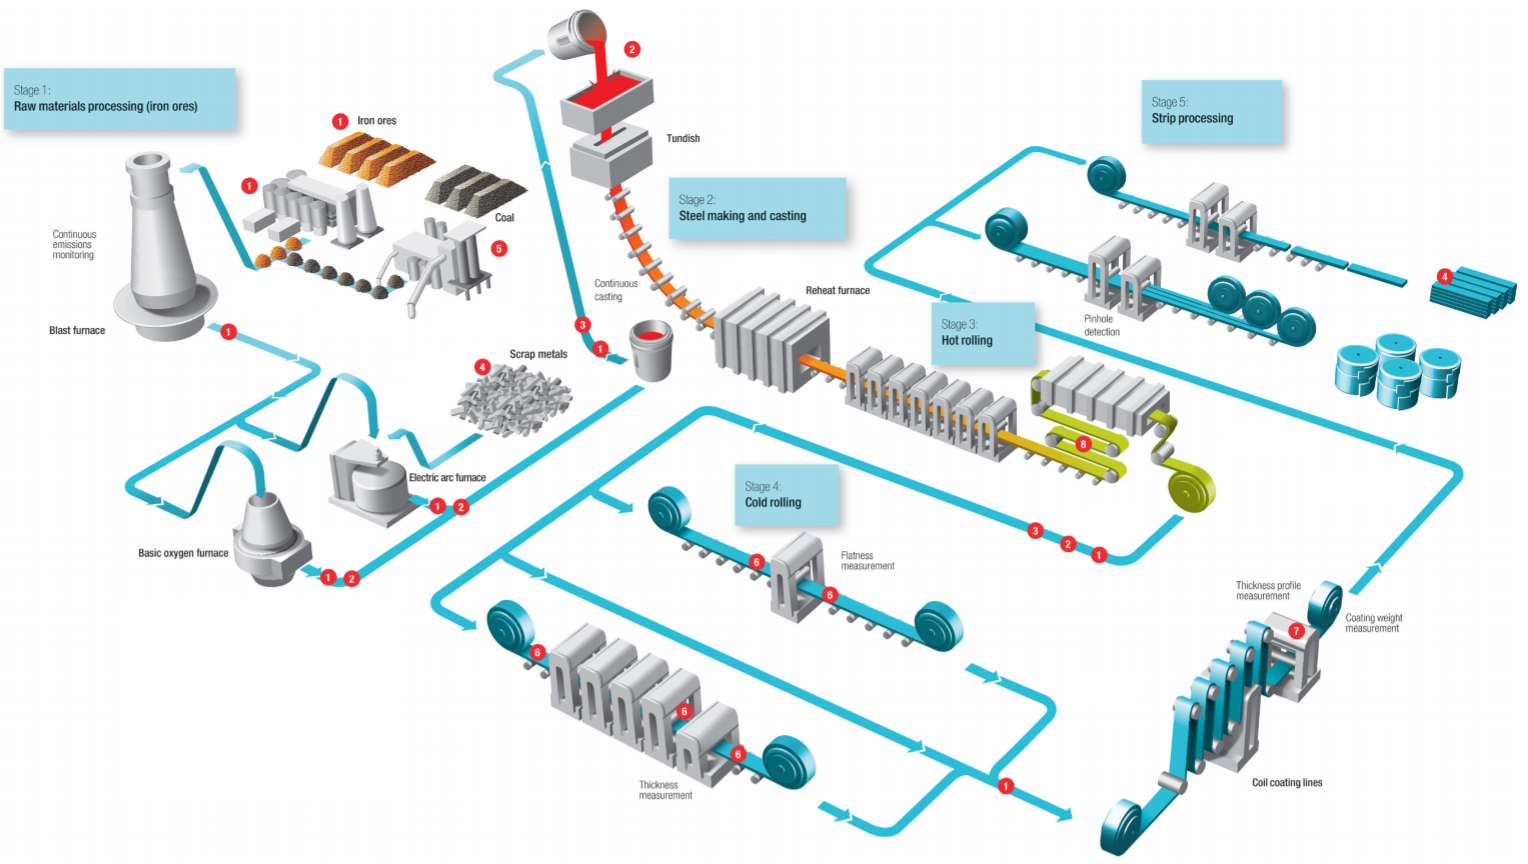
\includegraphics[width=1.0\linewidth]{../images/steel-production-steps.png}}
		\caption{Steel Manufacturing Steps~\cite{sinha-spinks_2015}.}
		\label{figure-steel-production-steps}
	\end{center}
\end{figure}

The above-explained processes and workstations can be arranged in various compact plant solutions based on the requirements of different facility organisations or demands. Table~\ref{Tab: production_lines} shows four separate production lines that the SMS group supplied to the steel manufacturing facility: Big River Steel, located in Arkansas, USA~\cite{BRS}.
\begin{table}[ht!]
	\centering
	\setlength{\arrayrulewidth}{0.75pt}% 
	\caption{Compact Production Lines with Various Machine Modules}
	\begin{tabular}{|c|c|c|}
		\hline
		\rowcolor[HTML]{FFFFC7} 
		\makecell{Label in\\Fig.~\ref{figure-steel-production-steps}} & Production Unit / Plant                       & Description                                                                                    \\ \hline
		A               & \makecell{Continuous Casting\\Machine (CCM)}            & \makecell{Mould steel cools and \\  solidifies, passing through \\the mould cavity.}                          \\ \hline
		B               & \makecell{Compact Strip \\Production (CSP)}              &\makecell{Compact plant including CCM,\\   reheating furnace, hot rolling unit \\and strip processing unit.}       \\ \hline
		C               & \makecell{Pickling Line \& Tandem \\Cold Mill (PLTCM)} & \makecell{Compact plant including a\\   turbulence pickling section \\and a tandem mill.}                     \\ \hline
		D               & \makecell{Continuous Galvanizing \\Line   (CGL)}         & \makecell{Application of protective zinc \\  coating on the steel surface to \\improve corrosion resistance.} \\ \hline
	\end{tabular}
	\label{Tab: production_lines}
\end{table}

Production lines given in Table~\ref{Tab: production_lines} are listed in the decreasing order for the product portfolio range. Many semi-finished products in various chemical and physical properties might be excluded from further production steps to be delivered to consumers right after casting and hot rolling units. As going further from CCM and CSP, the diversity of products gives its place to the more speciality among products in PLTCM and CGL.

 \begin{figure}[!ht]
	\begin{center}
		\makebox[\textwidth]{
			\centering
			\captionsetup{width=0.5\linewidth}
			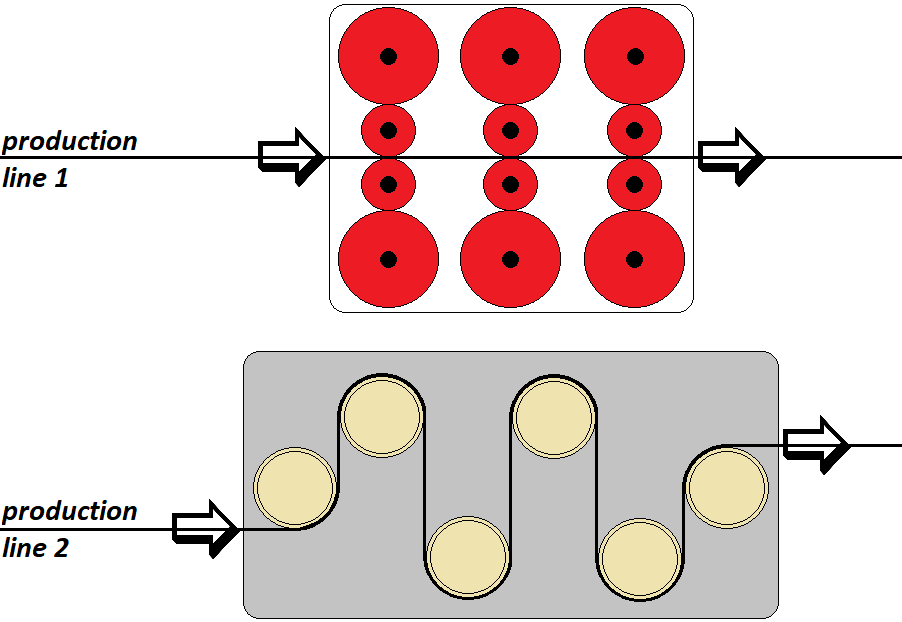
\includegraphics[width=0.9\linewidth]{../images/introduction-hypothetical_constraints.png}}
		\caption{Different Categories of Production Events Handling. The hot rolling mill positioned in production line 1 treats only one slab at a time. The unit in production line 2, pickling tank full of acid coloured in grey, treats the metal surface of more than one slab at a time.
		}
		\label{figure-hypothetical_constraints}
	\end{center}
\end{figure}

In addition to product range differences, one can also see the production style differs between those production lines. Fig.~\ref{figure-hypothetical_constraints} illustrates alternative handling categories for the production events in two separate production lines. Production events in the sequences need to be arranged in a specific order according to their width dimension~\cite{OZGUR2021106606}, which is a technical constraint belonging to the unit in production line 1. In contrast, there is no such technical constraint for the surface treatment; yet, a certain level of production events volume can be treated, bringing a load constraint on the unit in production line 2.

\section{Research Objective and Plan}

We argue that technology-driven constraints arise from the handling type in production line 1 introduced in Fig.~\ref{figure-hypothetical_constraints}. In contrast, the other kind of handling in production line 2 in the exact figure causes load-driven constraints. Moreover, the technology-driven constraints are effective in CCM and CSP, while the load-driven constraints are effective in PLTCM and CGL, in our opinion.

Outgrowing questioning leads to asking if those two fundamentally different constraints can be correctly discriminated with a formal definition and observe functional consequences related to that. Hypothesising alternative binning schemes for those constraints is a way of quantifying them and would allow us to investigate if they impact how the production system behaves.

As the first step, we constructed an analysis pipeline on steel production data concerning the identified binning schemes, which would provide us with the statistical impacts to discriminate the two types of constraints. We used Big River Steel production data belonging to the production lines introduced in Table~\ref{Tab: production_lines} among $2$--$3$ years and analysed it in time intervals to observe the statistical impacts. As the second step, we developed an abstract theoretical framework. We ran experimental simulations that would help understand the difference between those constraints mechanistically and their statistical patterns.

The two steps mentioned above constitutes our \ac{or} model, which combines steel production events analysis and constraint-based simulation. The art form of this model is to structure a standard data format and a shared analysis logic that allows comparing the results from steel production data and simulation data.